\usecaseristoratore{Segnalazione di un \textit{feedback}}
\label{usecase:Segnalazione di un feedback}

\begin{figure}[h]
	\centering
	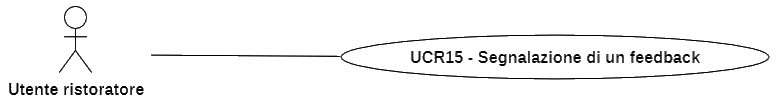
\includegraphics[width=0.8\textwidth]{./uml/UCR15.png} 
	\caption{Segnalazione di un \textit{feedback}}
	\label{fig:UCR15}
  \end{figure}

\begin{itemize}
	\item \textbf{Attore principale:} Utente ristoratore.

	\item \textbf{Precondizione:} L'Utente ristoratore è entrato nella sezione di consultazione dei \textit{feedback} relativi al suo ristorante.

	\item \textbf{Postcondizione:} L'Utente ristoratore segnala al Sistema che quel \textit{feedback} non è accettabile per determinate motivazioni.


	\item \textbf{Scenario principale:}
	      \begin{enumerate}
		      \item L'Utente ristoratore segnala al Sistema un \textit{feedback} che ritiene inopportuno;
		      \item L'Utente ristoratore inserisce le motivazioni della sua segnalazione;
		      \item Il Sistema registra la segnalazione del ristoratore.

	      \end{enumerate}
\end{itemize}
